%% fig_lefschetzgrid.tex   (generated by make_frontier.py; do not edit by hand)
%% The summands H^p(C,R^q) of an abelian scheme over a curve and the four operators of the proof.
\documentclass[tikz,border=8pt]{standalone}
\usepackage{amsmath,amssymb}
\usetikzlibrary{arrows.meta,calc,decorations.pathreplacing}
%% palette.tex -- shared colour definitions for the figures
\definecolor{PInk}{RGB}{26,32,44}
\definecolor{PBlue}{RGB}{37,82,139}
\definecolor{PTeal}{RGB}{23,127,125}
\definecolor{POchre}{RGB}{193,138,44}
\definecolor{PClay}{RGB}{178,74,58}
\definecolor{PSlate}{RGB}{108,122,137}
\definecolor{PViolet}{RGB}{110,86,150}
\definecolor{WBlue}{RGB}{223,234,246}
\definecolor{WTeal}{RGB}{220,238,236}
\definecolor{WOchre}{RGB}{250,240,218}
\definecolor{WClay}{RGB}{247,229,224}
\definecolor{WSlate}{RGB}{238,241,244}
\definecolor{PMag}{RGB}{158,58,110}
\definecolor{PGrass}{RGB}{62,124,66}
\definecolor{PAmber}{RGB}{214,112,38}
\definecolor{PIndigo}{RGB}{58,64,140}
\definecolor{PRule}{RGB}{176,186,197}

%% shared macros so the standalone figures match the paper
\providecommand{\QQ}{\mathbb{Q}}
\providecommand{\ZZ}{\mathbb{Z}}
\providecommand{\RR}{\mathbb{R}}
\providecommand{\CC}{\mathbb{C}}
\providecommand{\PP}{\mathbb{P}}
\providecommand{\Kx}{K^{\times}}
\providecommand{\HW}{W}
\providecommand{\Nm}{\mathrm{N}}
\providecommand{\Hdg}{\mathrm{Hdg}}
\providecommand{\NS}{\mathrm{NS}}
\providecommand{\cA}{\mathcal{A}}
\providecommand{\cD}{\mathcal{D}}
\providecommand{\cF}{\mathcal{F}}
\providecommand{\cP}{\mathcal{P}}
\providecommand{\cO}{\mathcal{O}}
\providecommand{\cQ}{\mathcal{Q}}
\providecommand{\bbar}[1]{\overline{#1}}
\providecommand{\ch}{\operatorname{ch}}
\providecommand{\End}{\mathrm{End}}

\newcommand{\hcimp}{\,\textcolor{PIndigo}{\tiny$\Leftarrow\mathbf{HC}$}}
\begin{document}
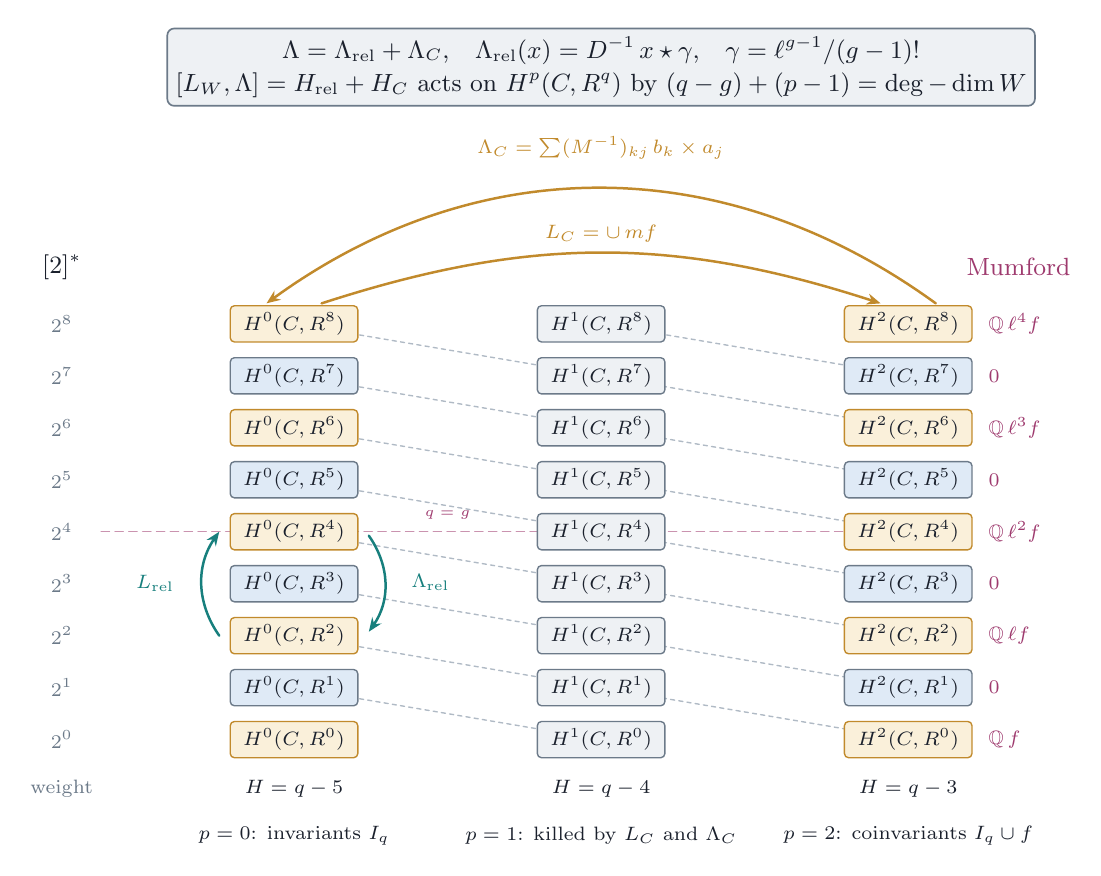
\begin{tikzpicture}[x=1cm,y=1cm,line join=round,line cap=round,
  font=\small,text=PInk]
  \draw[PMag!55,line width=0.50pt,dash pattern=on 3pt off 2pt] (-2.45,2.64) -- (8.62,2.64);
  \draw[PRule,line width=0.50pt,dash pattern=on 1.5pt off 1.5pt] (0.00,0.66) -- (3.90,0.00);
  \draw[PRule,line width=0.50pt,dash pattern=on 1.5pt off 1.5pt] (0.00,1.32) -- (3.90,0.66) -- (7.80,0.00);
  \draw[PRule,line width=0.50pt,dash pattern=on 1.5pt off 1.5pt] (0.00,1.98) -- (3.90,1.32) -- (7.80,0.66);
  \draw[PRule,line width=0.50pt,dash pattern=on 1.5pt off 1.5pt] (0.00,2.64) -- (3.90,1.98) -- (7.80,1.32);
  \draw[PRule,line width=0.50pt,dash pattern=on 1.5pt off 1.5pt] (0.00,3.30) -- (3.90,2.64) -- (7.80,1.98);
  \draw[PRule,line width=0.50pt,dash pattern=on 1.5pt off 1.5pt] (0.00,3.96) -- (3.90,3.30) -- (7.80,2.64);
  \draw[PRule,line width=0.50pt,dash pattern=on 1.5pt off 1.5pt] (0.00,4.62) -- (3.90,3.96) -- (7.80,3.30);
  \draw[PRule,line width=0.50pt,dash pattern=on 1.5pt off 1.5pt] (0.00,5.28) -- (3.90,4.62) -- (7.80,3.96);
  \draw[PRule,line width=0.50pt,dash pattern=on 1.5pt off 1.5pt] (3.90,5.28) -- (7.80,4.62);
  \node[draw=POchre,fill=WOchre,rounded corners=1.5pt,minimum width=1.62cm,minimum height=0.46cm,inner sep=1pt,line width=0.5pt] at (0.00,0.00) {\scriptsize $H^{0}(C,R^{0})$};
  \node[draw=PSlate,fill=WBlue,rounded corners=1.5pt,minimum width=1.62cm,minimum height=0.46cm,inner sep=1pt,line width=0.5pt] at (0.00,0.66) {\scriptsize $H^{0}(C,R^{1})$};
  \node[draw=POchre,fill=WOchre,rounded corners=1.5pt,minimum width=1.62cm,minimum height=0.46cm,inner sep=1pt,line width=0.5pt] at (0.00,1.32) {\scriptsize $H^{0}(C,R^{2})$};
  \node[draw=PSlate,fill=WBlue,rounded corners=1.5pt,minimum width=1.62cm,minimum height=0.46cm,inner sep=1pt,line width=0.5pt] at (0.00,1.98) {\scriptsize $H^{0}(C,R^{3})$};
  \node[draw=POchre,fill=WOchre,rounded corners=1.5pt,minimum width=1.62cm,minimum height=0.46cm,inner sep=1pt,line width=0.5pt] at (0.00,2.64) {\scriptsize $H^{0}(C,R^{4})$};
  \node[draw=PSlate,fill=WBlue,rounded corners=1.5pt,minimum width=1.62cm,minimum height=0.46cm,inner sep=1pt,line width=0.5pt] at (0.00,3.30) {\scriptsize $H^{0}(C,R^{5})$};
  \node[draw=POchre,fill=WOchre,rounded corners=1.5pt,minimum width=1.62cm,minimum height=0.46cm,inner sep=1pt,line width=0.5pt] at (0.00,3.96) {\scriptsize $H^{0}(C,R^{6})$};
  \node[draw=PSlate,fill=WBlue,rounded corners=1.5pt,minimum width=1.62cm,minimum height=0.46cm,inner sep=1pt,line width=0.5pt] at (0.00,4.62) {\scriptsize $H^{0}(C,R^{7})$};
  \node[draw=POchre,fill=WOchre,rounded corners=1.5pt,minimum width=1.62cm,minimum height=0.46cm,inner sep=1pt,line width=0.5pt] at (0.00,5.28) {\scriptsize $H^{0}(C,R^{8})$};
  \node[draw=PSlate,fill=WSlate,rounded corners=1.5pt,minimum width=1.62cm,minimum height=0.46cm,inner sep=1pt,line width=0.5pt] at (3.90,0.00) {\scriptsize $H^{1}(C,R^{0})$};
  \node[draw=PSlate,fill=WSlate,rounded corners=1.5pt,minimum width=1.62cm,minimum height=0.46cm,inner sep=1pt,line width=0.5pt] at (3.90,0.66) {\scriptsize $H^{1}(C,R^{1})$};
  \node[draw=PSlate,fill=WSlate,rounded corners=1.5pt,minimum width=1.62cm,minimum height=0.46cm,inner sep=1pt,line width=0.5pt] at (3.90,1.32) {\scriptsize $H^{1}(C,R^{2})$};
  \node[draw=PSlate,fill=WSlate,rounded corners=1.5pt,minimum width=1.62cm,minimum height=0.46cm,inner sep=1pt,line width=0.5pt] at (3.90,1.98) {\scriptsize $H^{1}(C,R^{3})$};
  \node[draw=PSlate,fill=WSlate,rounded corners=1.5pt,minimum width=1.62cm,minimum height=0.46cm,inner sep=1pt,line width=0.5pt] at (3.90,2.64) {\scriptsize $H^{1}(C,R^{4})$};
  \node[draw=PSlate,fill=WSlate,rounded corners=1.5pt,minimum width=1.62cm,minimum height=0.46cm,inner sep=1pt,line width=0.5pt] at (3.90,3.30) {\scriptsize $H^{1}(C,R^{5})$};
  \node[draw=PSlate,fill=WSlate,rounded corners=1.5pt,minimum width=1.62cm,minimum height=0.46cm,inner sep=1pt,line width=0.5pt] at (3.90,3.96) {\scriptsize $H^{1}(C,R^{6})$};
  \node[draw=PSlate,fill=WSlate,rounded corners=1.5pt,minimum width=1.62cm,minimum height=0.46cm,inner sep=1pt,line width=0.5pt] at (3.90,4.62) {\scriptsize $H^{1}(C,R^{7})$};
  \node[draw=PSlate,fill=WSlate,rounded corners=1.5pt,minimum width=1.62cm,minimum height=0.46cm,inner sep=1pt,line width=0.5pt] at (3.90,5.28) {\scriptsize $H^{1}(C,R^{8})$};
  \node[draw=POchre,fill=WOchre,rounded corners=1.5pt,minimum width=1.62cm,minimum height=0.46cm,inner sep=1pt,line width=0.5pt] at (7.80,0.00) {\scriptsize $H^{2}(C,R^{0})$};
  \node[draw=PSlate,fill=WBlue,rounded corners=1.5pt,minimum width=1.62cm,minimum height=0.46cm,inner sep=1pt,line width=0.5pt] at (7.80,0.66) {\scriptsize $H^{2}(C,R^{1})$};
  \node[draw=POchre,fill=WOchre,rounded corners=1.5pt,minimum width=1.62cm,minimum height=0.46cm,inner sep=1pt,line width=0.5pt] at (7.80,1.32) {\scriptsize $H^{2}(C,R^{2})$};
  \node[draw=PSlate,fill=WBlue,rounded corners=1.5pt,minimum width=1.62cm,minimum height=0.46cm,inner sep=1pt,line width=0.5pt] at (7.80,1.98) {\scriptsize $H^{2}(C,R^{3})$};
  \node[draw=POchre,fill=WOchre,rounded corners=1.5pt,minimum width=1.62cm,minimum height=0.46cm,inner sep=1pt,line width=0.5pt] at (7.80,2.64) {\scriptsize $H^{2}(C,R^{4})$};
  \node[draw=PSlate,fill=WBlue,rounded corners=1.5pt,minimum width=1.62cm,minimum height=0.46cm,inner sep=1pt,line width=0.5pt] at (7.80,3.30) {\scriptsize $H^{2}(C,R^{5})$};
  \node[draw=POchre,fill=WOchre,rounded corners=1.5pt,minimum width=1.62cm,minimum height=0.46cm,inner sep=1pt,line width=0.5pt] at (7.80,3.96) {\scriptsize $H^{2}(C,R^{6})$};
  \node[draw=PSlate,fill=WBlue,rounded corners=1.5pt,minimum width=1.62cm,minimum height=0.46cm,inner sep=1pt,line width=0.5pt] at (7.80,4.62) {\scriptsize $H^{2}(C,R^{7})$};
  \node[draw=POchre,fill=WOchre,rounded corners=1.5pt,minimum width=1.62cm,minimum height=0.46cm,inner sep=1pt,line width=0.5pt] at (7.80,5.28) {\scriptsize $H^{2}(C,R^{8})$};
  \node[text=PInk,inner sep=1pt,align=center,font=\small] at (-2.95,6.00) {$[2]^{*}$};
  \node[text=PSlate,inner sep=1pt,align=center,font=\scriptsize] at (-2.95,0.00) {$2^{0}$};
  \node[text=PSlate,inner sep=1pt,align=center,font=\scriptsize] at (-2.95,0.66) {$2^{1}$};
  \node[text=PSlate,inner sep=1pt,align=center,font=\scriptsize] at (-2.95,1.32) {$2^{2}$};
  \node[text=PSlate,inner sep=1pt,align=center,font=\scriptsize] at (-2.95,1.98) {$2^{3}$};
  \node[text=PSlate,inner sep=1pt,align=center,font=\scriptsize] at (-2.95,2.64) {$2^{4}$};
  \node[text=PSlate,inner sep=1pt,align=center,font=\scriptsize] at (-2.95,3.30) {$2^{5}$};
  \node[text=PSlate,inner sep=1pt,align=center,font=\scriptsize] at (-2.95,3.96) {$2^{6}$};
  \node[text=PSlate,inner sep=1pt,align=center,font=\scriptsize] at (-2.95,4.62) {$2^{7}$};
  \node[text=PSlate,inner sep=1pt,align=center,font=\scriptsize] at (-2.95,5.28) {$2^{8}$};
  \node[text=PSlate,inner sep=1pt,align=center,font=\scriptsize] at (-2.95,-0.62) {weight};
  \node[text=PInk,inner sep=1pt,align=center,font=\scriptsize] at (0.00,-0.62) {$H=q-5$};
  \node[text=PInk,inner sep=1pt,align=center,font=\scriptsize] at (3.90,-0.62) {$H=q-4$};
  \node[text=PInk,inner sep=1pt,align=center,font=\scriptsize] at (7.80,-0.62) {$H=q-3$};
  \node[text=PInk,inner sep=1pt,align=center,font=\scriptsize] at (0.00,-1.22) {$p=0$: invariants $I_{q}$};
  \node[text=PInk,inner sep=1pt,align=center,font=\scriptsize] at (3.90,-1.22) {$p=1$: killed by $L_{C}$ and $\Lambda_{C}$};
  \node[text=PInk,inner sep=1pt,align=center,font=\scriptsize] at (7.80,-1.22) {$p=2$: coinvariants $I_{q}\cup f$};
  \draw[PTeal,line width=0.90pt,-{Stealth[length=5pt,width=4pt]},bend left=35] (-0.95,1.32) to (-0.95,2.64);
  \draw[PTeal,line width=0.90pt,-{Stealth[length=5pt,width=4pt]},bend left=35] (0.95,2.59) to (0.95,1.37);
  \node[text=PTeal,inner sep=1pt,align=center,font=\scriptsize,anchor=east] at (-1.48,1.98) {$L_{\mathrm{rel}}$};
  \node[text=PTeal,inner sep=1pt,align=center,font=\scriptsize,anchor=west] at (1.45,2.00) {$\Lambda_{\mathrm{rel}}$};
  \draw[POchre,line width=0.90pt,-{Stealth[length=5pt,width=4pt]},bend left=18] (0.35,5.54) to (7.45,5.54);
  \draw[POchre,line width=0.90pt,-{Stealth[length=5pt,width=4pt]},bend right=36] (8.15,5.54) to (-0.35,5.54);
  \node[text=POchre,inner sep=1pt,align=center,font=\scriptsize] at (3.90,6.42) {$L_{C}=\cup\,mf$};
  \node[text=POchre,inner sep=1pt,align=center,font=\scriptsize] at (3.90,7.52) {$\Lambda_{C}=\sum(M^{-1})_{kj}\,b_{k}\times a_{j}$};
  \node[draw=PSlate,fill=WSlate,rounded corners=2.5pt,inner sep=3pt,line width=0.60pt,align=center] at (3.90,8.54) {$\Lambda=\Lambda_{\mathrm{rel}}+\Lambda_{C}$,\quad $\Lambda_{\mathrm{rel}}(x)=D^{-1}\,x\star\gamma$,\quad $\gamma=\ell^{g-1}/(g-1)!$\\[1pt]$[L_{W},\Lambda]=H_{\mathrm{rel}}+H_{C}$ acts on $H^{p}(C,R^{q})$ by $(q-g)+(p-1)=\deg-\dim W$};
  \node[text=PMag,inner sep=1pt,align=center,font=\small] at (9.20,6.00) {Mumford};
  \node[text=PMag,inner sep=1pt,align=center,font=\scriptsize,anchor=west] at (8.78,0.00) {$\QQ\,f$};
  \node[text=PMag,inner sep=1pt,align=center,font=\scriptsize,anchor=west] at (8.78,0.66) {$0$};
  \node[text=PMag,inner sep=1pt,align=center,font=\scriptsize,anchor=west] at (8.78,1.32) {$\QQ\,\ell f$};
  \node[text=PMag,inner sep=1pt,align=center,font=\scriptsize,anchor=west] at (8.78,1.98) {$0$};
  \node[text=PMag,inner sep=1pt,align=center,font=\scriptsize,anchor=west] at (8.78,2.64) {$\QQ\,\ell^{2}f$};
  \node[text=PMag,inner sep=1pt,align=center,font=\scriptsize,anchor=west] at (8.78,3.30) {$0$};
  \node[text=PMag,inner sep=1pt,align=center,font=\scriptsize,anchor=west] at (8.78,3.96) {$\QQ\,\ell^{3}f$};
  \node[text=PMag,inner sep=1pt,align=center,font=\scriptsize,anchor=west] at (8.78,4.62) {$0$};
  \node[text=PMag,inner sep=1pt,align=center,font=\scriptsize,anchor=west] at (8.78,5.28) {$\QQ\,\ell^{4}f$};
  \node[text=PMag,inner sep=1pt,align=center,font=\tiny] at (1.95,2.86) {$q=g$};
\end{tikzpicture}
\end{document}
